\chapter{Acercamientos Previos a la Soluci\'on}

\section{Est\'atico: m\'axima ganancia posible}

Si la demanda del consumidor no var\'ia, la soluci\'on es cerrada y puede encontrarse de la siguiente manera:

\section{Estacional y aleatorio: m\'as parecido al mundo real}

En el mundo real, ning\'un producto tiene una demanda perfectamente constante. M\'as a\'un, existen una infinidad de productos cuya demanda var\'ia con un patr\'on estacional: por ejemplo, las medicinas antigripales se venden m\'as en invierno. La cerveza (y, en general, las bebidas alcoh\'olicas) tambi\'en siguen este tipo de patrones.\\

En primer lugar, existe un patr\'on semanal bastante esperado: seg\'un \citet{}, se consume m\'as cerveza los fines de semana (ver la figura \ref{weekly_base}). Adem\'as, existe un patr\'on relacionado a las festividades comunes. Seg\'un \citet{}, el consumo de bebidas alcoh\'olicas se duplica en las festividades navide\~nas. \\

\begin{figure}[h]
\caption{ }
\label{weekly_base}
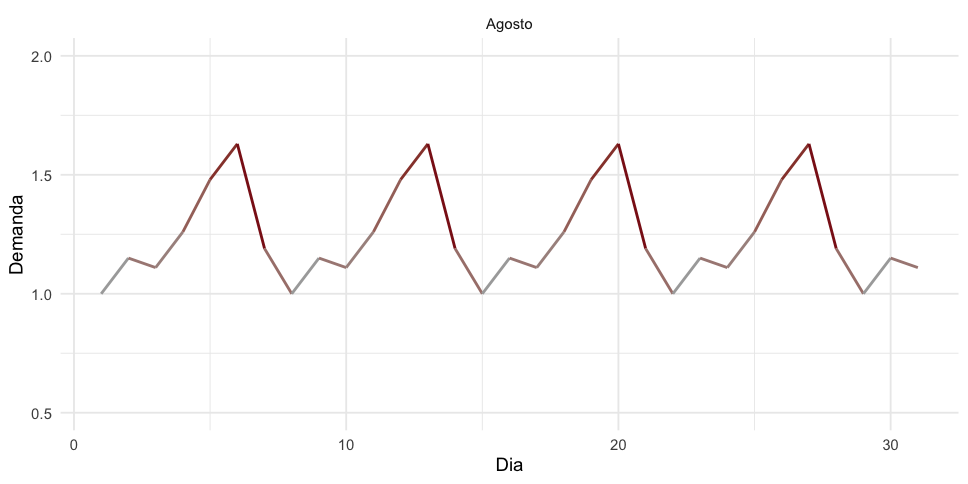
\includegraphics[width=15cm]{monthly_customer_demand_ggplot.png}
\centering
\end{figure}

Para el presente trabajo, combinaremos los dos patrones descritos anteriormente, y a\~nadiremos un peque\~no componente aleatorio que cambiar\'a la demanda cada a\~no. El comportamiento ''base'' de la demanda de puede consultar en la figura \ref{yearly_base}. Sin embargo, cabe mencionar que este es un modelo simple, pues en algunas regiones, podr\'ia tambi\'en existir un patr\'on relacionado al clima, o incluso un alza en la demanda siguiendo temporadas deportivas. \\

\begin{figure}[h]
\caption{ }
\label{yearly_base}
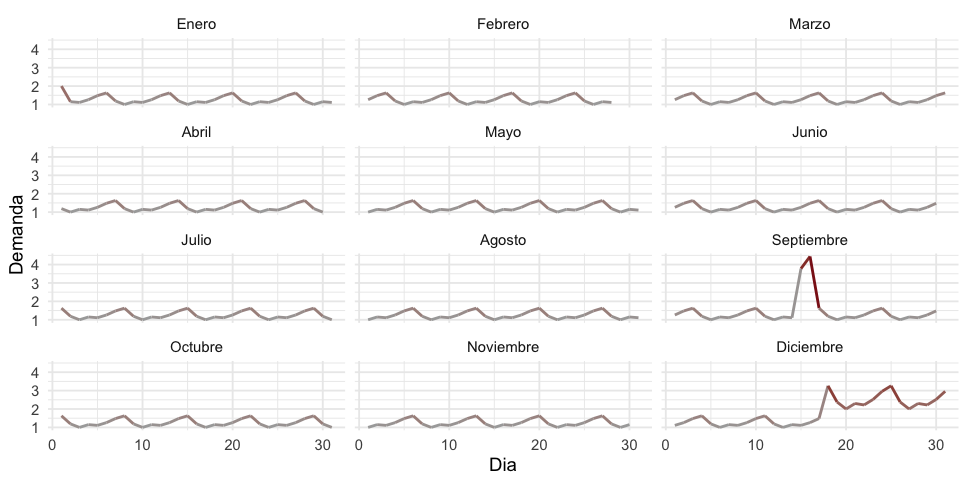
\includegraphics[width=15cm]{monthly_demand_ggplot.png}
\centering
\end{figure}

Como el comportamiento var\'ia a lo largo del a\~no y existe un costo por almacenar inventario, cada agente debe prepararse con adecuada anticipaci\'on para los picos de demanda. Adem\'as, el componente aleatorio resulta en la necesidad de conservar inventario de seguridad (en ingl\'es, \textit{safety stock}) para asegurar que la demanda ser\'a cubierta la mayor parte del tiempo.

\section{Q-Learning}
Aqu\'i hablar del paper que encontr\'e que hace QL \citet{Chaharsooghi}

Sin embargo, ninguna de estas soluciones considera la restricción de temporalidad de producci\'on de materias primas. En el siguiente cap\'itulo, se presentar\'a este escenario como un nivel extra de complejidad al modelo, limitando la oferta de cebada por parte de los campos.